\documentclass[border=5pt]{standalone}
\usepackage{fontspec}
\usepackage{unicode-math}
\setmainfont{Noto Serif}
\newfontfamily\FigureItalic{Noto Serif}
\setmathfont{STIXTwoMath-Regular.otf}
\usepackage{tikz}
\usetikzlibrary{arrows.meta,calc,patterns,decorations.pathmorphing,decorations.markings,decorations.pathreplacing,positioning,backgrounds}
\definecolor{Ink}{HTML}{000000}
\definecolor{Curve}{HTML}{000000}
\definecolor{Bzero}{HTML}{000000}
\definecolor{Bone}{HTML}{000000}
\definecolor{Btwo}{HTML}{000000}
\definecolor{Bthree}{HTML}{000000}
\definecolor{Bfour}{HTML}{000000}
\tikzset{
 ax/.style={draw=Ink,line width=.72pt,-{Latex[length=2.4mm,width=1.5mm]}},
 lev/.style={draw=Ink,line width=1.4pt,line cap=butt},
 thinlev/.style={draw=Ink,line width=.65pt,line cap=butt},
 helper/.style={draw=Ink,line width=.65pt},
 bare/.style={draw=Ink,line width=.95pt,dash pattern=on 4pt off 2.8pt},
 curve/.style={draw=Ink,line width=1.85pt,line cap=round,line join=round},
 ray/.style={draw=Ink,line width=1.0pt,-{Latex[length=2.3mm,width=1.4mm]}},
 measure/.style={draw=Ink,line width=.75pt,{Latex[length=1.9mm,width=1.2mm]}-{Latex[length=1.9mm,width=1.2mm]}},
 link/.style={draw=Ink,line width=1.0pt},
 wave/.style={draw=Ink,line width=.85pt,decorate,decoration={snake,amplitude=.33mm,segment length=2.5mm,pre length=.8mm,post length=.8mm}},
 photon/.style={draw=Ink,line width=1.0pt,-{Latex[length=2.0mm,width=1.3mm]},decorate,decoration={snake,amplitude=.4mm,segment length=2.7mm,pre length=0mm,post length=1.9mm}},
 lab/.style={text=Ink,font=\fontsize{13.5}{16}\selectfont,inner sep=2pt},
 small/.style={text=Ink,font=\fontsize{11.5}{14}\selectfont,inner sep=2pt},
 tag/.style={text=Ink,font=\fontsize{14}{17}\selectfont\FigureItalic\itshape,inner sep=2pt}}
\pagestyle{empty}

\begin{document}
% Figure 13.3; source-grounded revision.
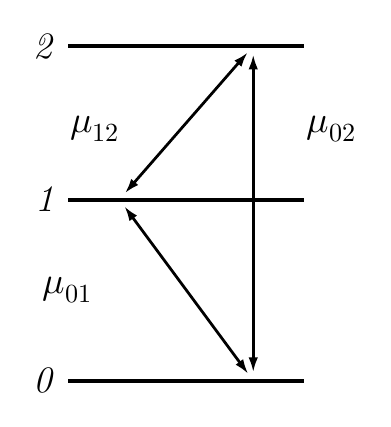
\begin{tikzpicture}[x=1cm,y=1cm]
\coordinate (e0) at (2.40000,0.00000);
\coordinate (e0L) at (0.90000,0.00000);
\coordinate (e0R) at (3.90000,0.00000);
\draw[lev] (e0L) -- (e0R);
\node[lab,anchor=east] at (0.80000,0.00000) {\textit{0}};
\coordinate (e1) at (2.40000,2.30000);
\coordinate (e1L) at (0.90000,2.30000);
\coordinate (e1R) at (3.90000,2.30000);
\draw[lev] (e1L) -- (e1R);
\node[lab,anchor=east] at (0.80000,2.30000) {\textit{1}};
\coordinate (e2) at (2.40000,4.25000);
\coordinate (e2L) at (0.90000,4.25000);
\coordinate (e2R) at (3.90000,4.25000);
\draw[lev] (e2L) -- (e2R);
\node[lab,anchor=east] at (0.80000,4.25000) {\textit{2}};
\coordinate (P0) at (3.25000,0.00000);
\coordinate (P1) at (1.55000,2.30000);
\coordinate (P2) at (3.25000,4.25000);
\draw[measure,line width=1pt,shorten <=3pt,shorten >=3pt] (P0) -- (P1);
\node[lab] at (0.90000,1.15000) {$\mu_{01}$};
\draw[measure,line width=1pt,shorten <=3pt,shorten >=3pt] (P1) -- (P2);
\node[lab] at (1.25000,3.20000) {$\mu_{12}$};
\draw[measure,line width=1pt,shorten <=3pt,shorten >=3pt] (P0) -- (P2);
\node[lab] at (4.25000,3.20000) {$\mu_{02}$};\end{tikzpicture}

\end{document}
